\documentclass[tikz,border=8pt]{standalone}
% Shared look for every TikZ diagram. Load with \input{../../tools/tikz-style.tex}
\usepackage[sfdefault]{roboto}
\usetikzlibrary{arrows.meta, positioning, shapes.geometric, calc, fit, backgrounds}
\definecolor{cblue}{HTML}{4C78A8}
\definecolor{corange}{HTML}{F58518}
\definecolor{cgreen}{HTML}{54A24B}
\definecolor{cred}{HTML}{E45756}
\definecolor{cpurple}{HTML}{B279A2}
\definecolor{cgrey}{HTML}{6B6B6B}
\tikzset{
  every picture/.style={font=\sffamily, line width=1.2pt},
  box/.style={draw=#1, fill=#1!12, rounded corners=4pt, align=center, inner sep=7pt, minimum height=1.1cm},
  box/.default=cgrey,
  arrow/.style={-{Stealth[length=3mm]}, draw=cgrey, line width=1.4pt},
  title/.style={font=\sffamily\bfseries\Large},
  note/.style={font=\sffamily\small, text=cgrey, align=center},
}
\AtBeginDocument{\hyphenpenalty=10000 \exhyphenpenalty=10000}

% The arc through the look-ahead point, in the car's frame at the start (x forward, y left, origin at the rear axle).
% Look-ahead point G = (3.873, -1); the arc is tangent to the heading at the rear axle, so its centre C lies on the
% rear-axle line (the y axis), at (0, R) with R = -8 m. Triangle C, F = (0, -1), G: legs 7 m and 3.873 m,
% hypotenuse 8 m (49 + 15 = 64). The chord from the rear axle to G is the look-ahead distance, 4 m;
% alpha = -14.48 deg. 1 unit = 1 m.
\begin{document}
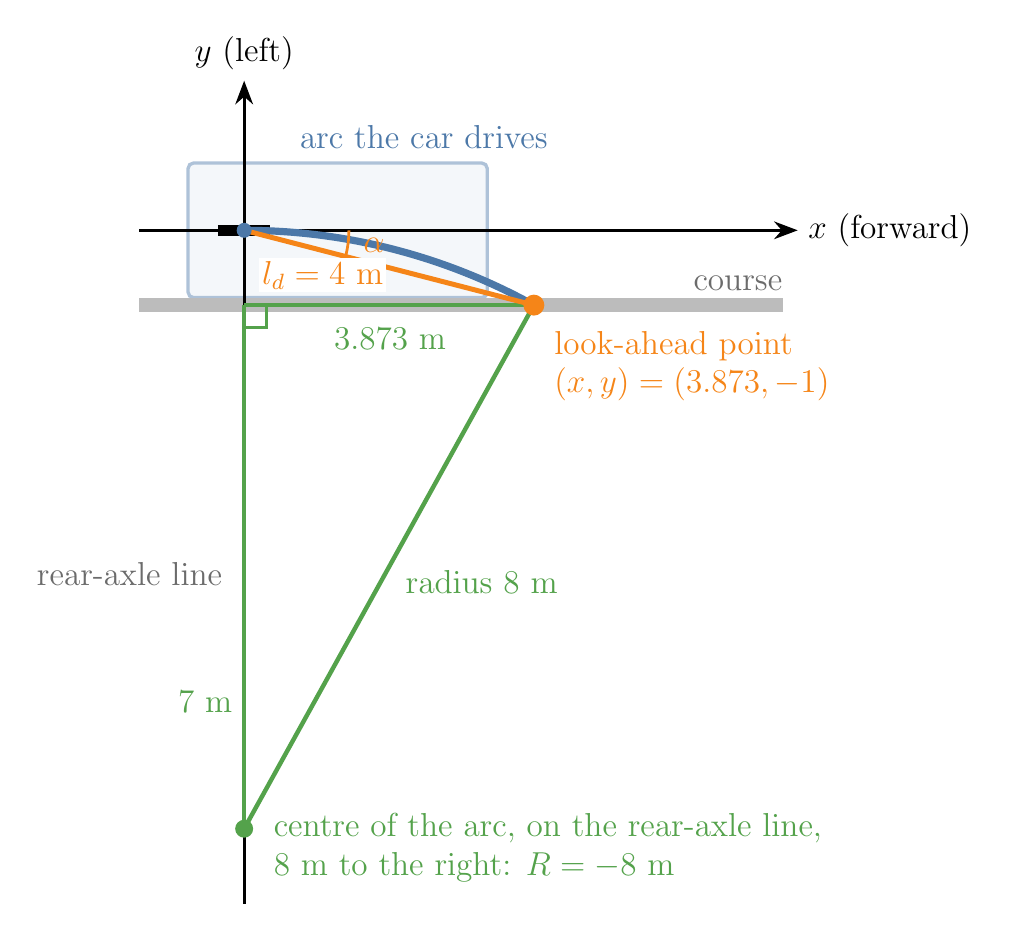
\begin{tikzpicture}[scale=0.95, every node/.append style={font=\large}]
  % faint car body at the origin
  \draw[cblue!45, fill=cblue!6, rounded corners=2pt] (-0.75,-0.9) rectangle (3.25,0.9);
  \draw[black, line width=4pt] (-0.35,0) -- (0.35,0);
  % course
  \draw[cgrey!45, line width=5pt] (-1.4,-1) -- (7.2,-1);
  \node[cgrey, anchor=south] at (6.6,-0.95) {course};
  % axes: x forward, y left (the rear-axle line)
  \draw[-{Stealth[length=3mm]}, black, line width=1pt] (-1.4,0) -- (7.4,0) node[right] {$x$ (forward)};
  \draw[-{Stealth[length=3mm]}, black, line width=1pt] (0,-9.0) -- (0,2.0) node[above] {$y$ (left)};
  \node[cgrey, anchor=east, align=right] at (-0.15,-4.6) {rear-axle line};
  % the circle the car would drive, and the arc to the look-ahead point
  \draw[cblue, line width=2.6pt] (0,0) arc[start angle=90, end angle=61.05, radius=8];
  \node[cblue, anchor=south west] at (0.6,0.95) {arc the car drives};
  % triangle C, F, G
  \coordinate (C) at (0,-8); \coordinate (F) at (0,-1); \coordinate (G) at (3.873,-1);
  \draw[cgreen, line width=1.6pt] (C) -- (G);
  \draw[cgreen, line width=1.6pt] (C) -- (F);
  \draw[cgreen, line width=1.6pt] (F) -- (G);
  \draw[cgreen, line width=1pt] (0.3,-1) -- (0.3,-1.3) -- (0,-1.3);
  \node[cgreen, anchor=east, fill=white, inner sep=1pt] at (-0.1,-6.3) {7 m};
  \node[cgreen, anchor=north, fill=white, inner sep=1pt] at (1.95,-1.25) {3.873 m};
  \node[cgreen, anchor=west, fill=white, inner sep=1pt] at (2.1,-4.7) {radius 8 m};
  \fill[cgreen] (C) circle (0.12);
  \node[cgreen, anchor=west, align=left] at (0.25,-8.25) {centre of the arc, on the rear-axle line,\\8 m to the right: $R = -8$ m};
  % chord = look-ahead distance, and alpha
  \draw[corange, line width=1.8pt] (0,0) -- (G);
  \node[corange, fill=white, inner sep=1pt] at (1.05,-0.6) {$l_d = 4$ m};
  \draw[corange, line width=1pt] (1.4,0) arc[start angle=0, end angle=-14.48, radius=1.4];
  \node[corange, anchor=west] at (1.45,-0.2) {$\alpha$};
  \fill[corange] (G) circle (0.14);
  \node[corange, anchor=north west, align=left] at (4.0,-1.2) {look-ahead point\\$(x, y) = (3.873, -1)$};
  \fill[cblue] (0,0) circle (0.1);
\end{tikzpicture}
\end{document}
